\begin{center}
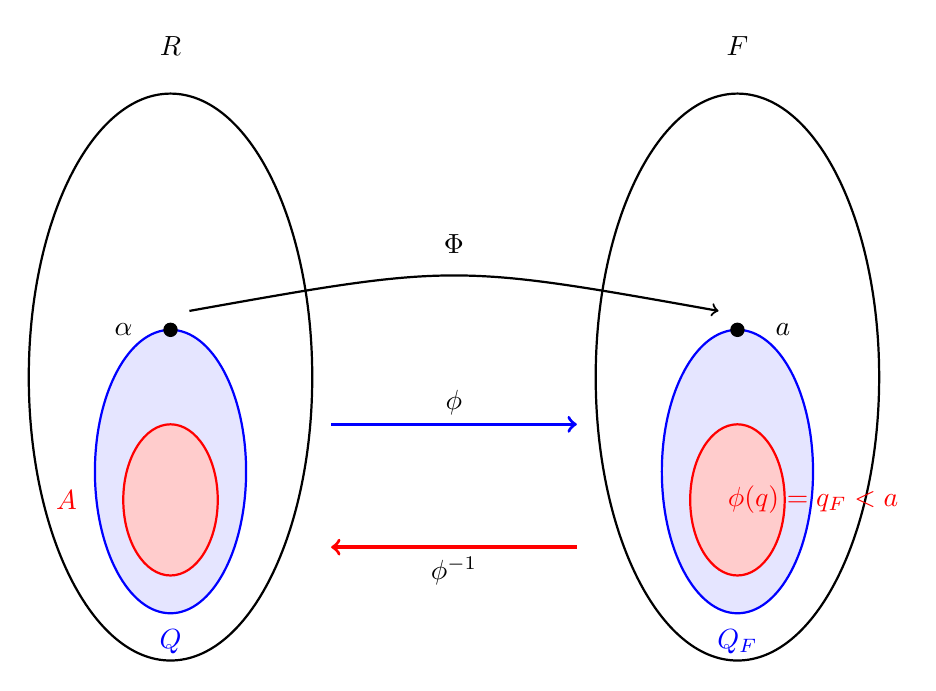
\begin{tikzpicture}[scale=1.2]
    % Left set (R)
    \draw[thick] (-2,0) ellipse (1.5cm and 3cm);
    \node at (-2, 3.5) {$\mathbb{R}$};
    
    % Right set (F)
    \draw[thick] (4,0) ellipse (1.5cm and 3cm);
    \node at (4, 3.5) {$\mathbb{F}$};
    
    % Rationals in R (highlighted region)
    \draw[thick, blue, fill=blue!10] (-2,-1) ellipse (0.8cm and 1.5cm);
    \node[blue] at (-2, -2.8) {$\mathbb{Q}$};
    
    % Rationals in F (highlighted region)
    \draw[thick, blue, fill=blue!10] (4,-1) ellipse (0.8cm and 1.5cm);
    \node[blue] at (4, -2.8) {$\mathbb{Q}_F$};
    
    % Set A (the preimage)
    \draw[thick, red, fill=red!20] (-2,-1.3) ellipse (0.5cm and 0.8cm);
    \node[red] at (-3.1, -1.3) {$A$};
    
    % Elements below a in Q_F
    \draw[thick, red, fill=red!20] (4,-1.3) ellipse (0.5cm and 0.8cm);
    \node[red] at (4.8, -1.3) {$\phi(q) = q_\mathbb{F} < a$};
    
    % Alpha (supremum of A)
    \filldraw[black] (-2, 0.5) circle (2pt);
    \node[left] at (-2.3, 0.5) {$\alpha$};
    
    % a in F
    \filldraw[black] (4, 0.5) circle (2pt);
    \node[right] at (4.3, 0.5) {$a$};
    
    % Phi arrow (forward)
    \draw[->, very thick, blue] (-0.3, -0.5) -- (2.3, -0.5);
    \node[above] at (1, -0.5) {$\phi$};
    
    % Phi inverse arrow (backward)
    \draw[->, very thick, red] (2.3, -1.8) -- (-0.3, -1.8);
    \node[below] at (1, -1.8) {$\phi^{-1}$};
    
    % Phi arrow from alpha to a
    \draw[->, thick, black] (-1.8, 0.7) .. controls (1, 1.2) .. (3.8, 0.7);
    \node[above] at (1, 1.2) {$\Phi$};
\end{tikzpicture}
\end{center}
